\section{Results}

\begin{center}
   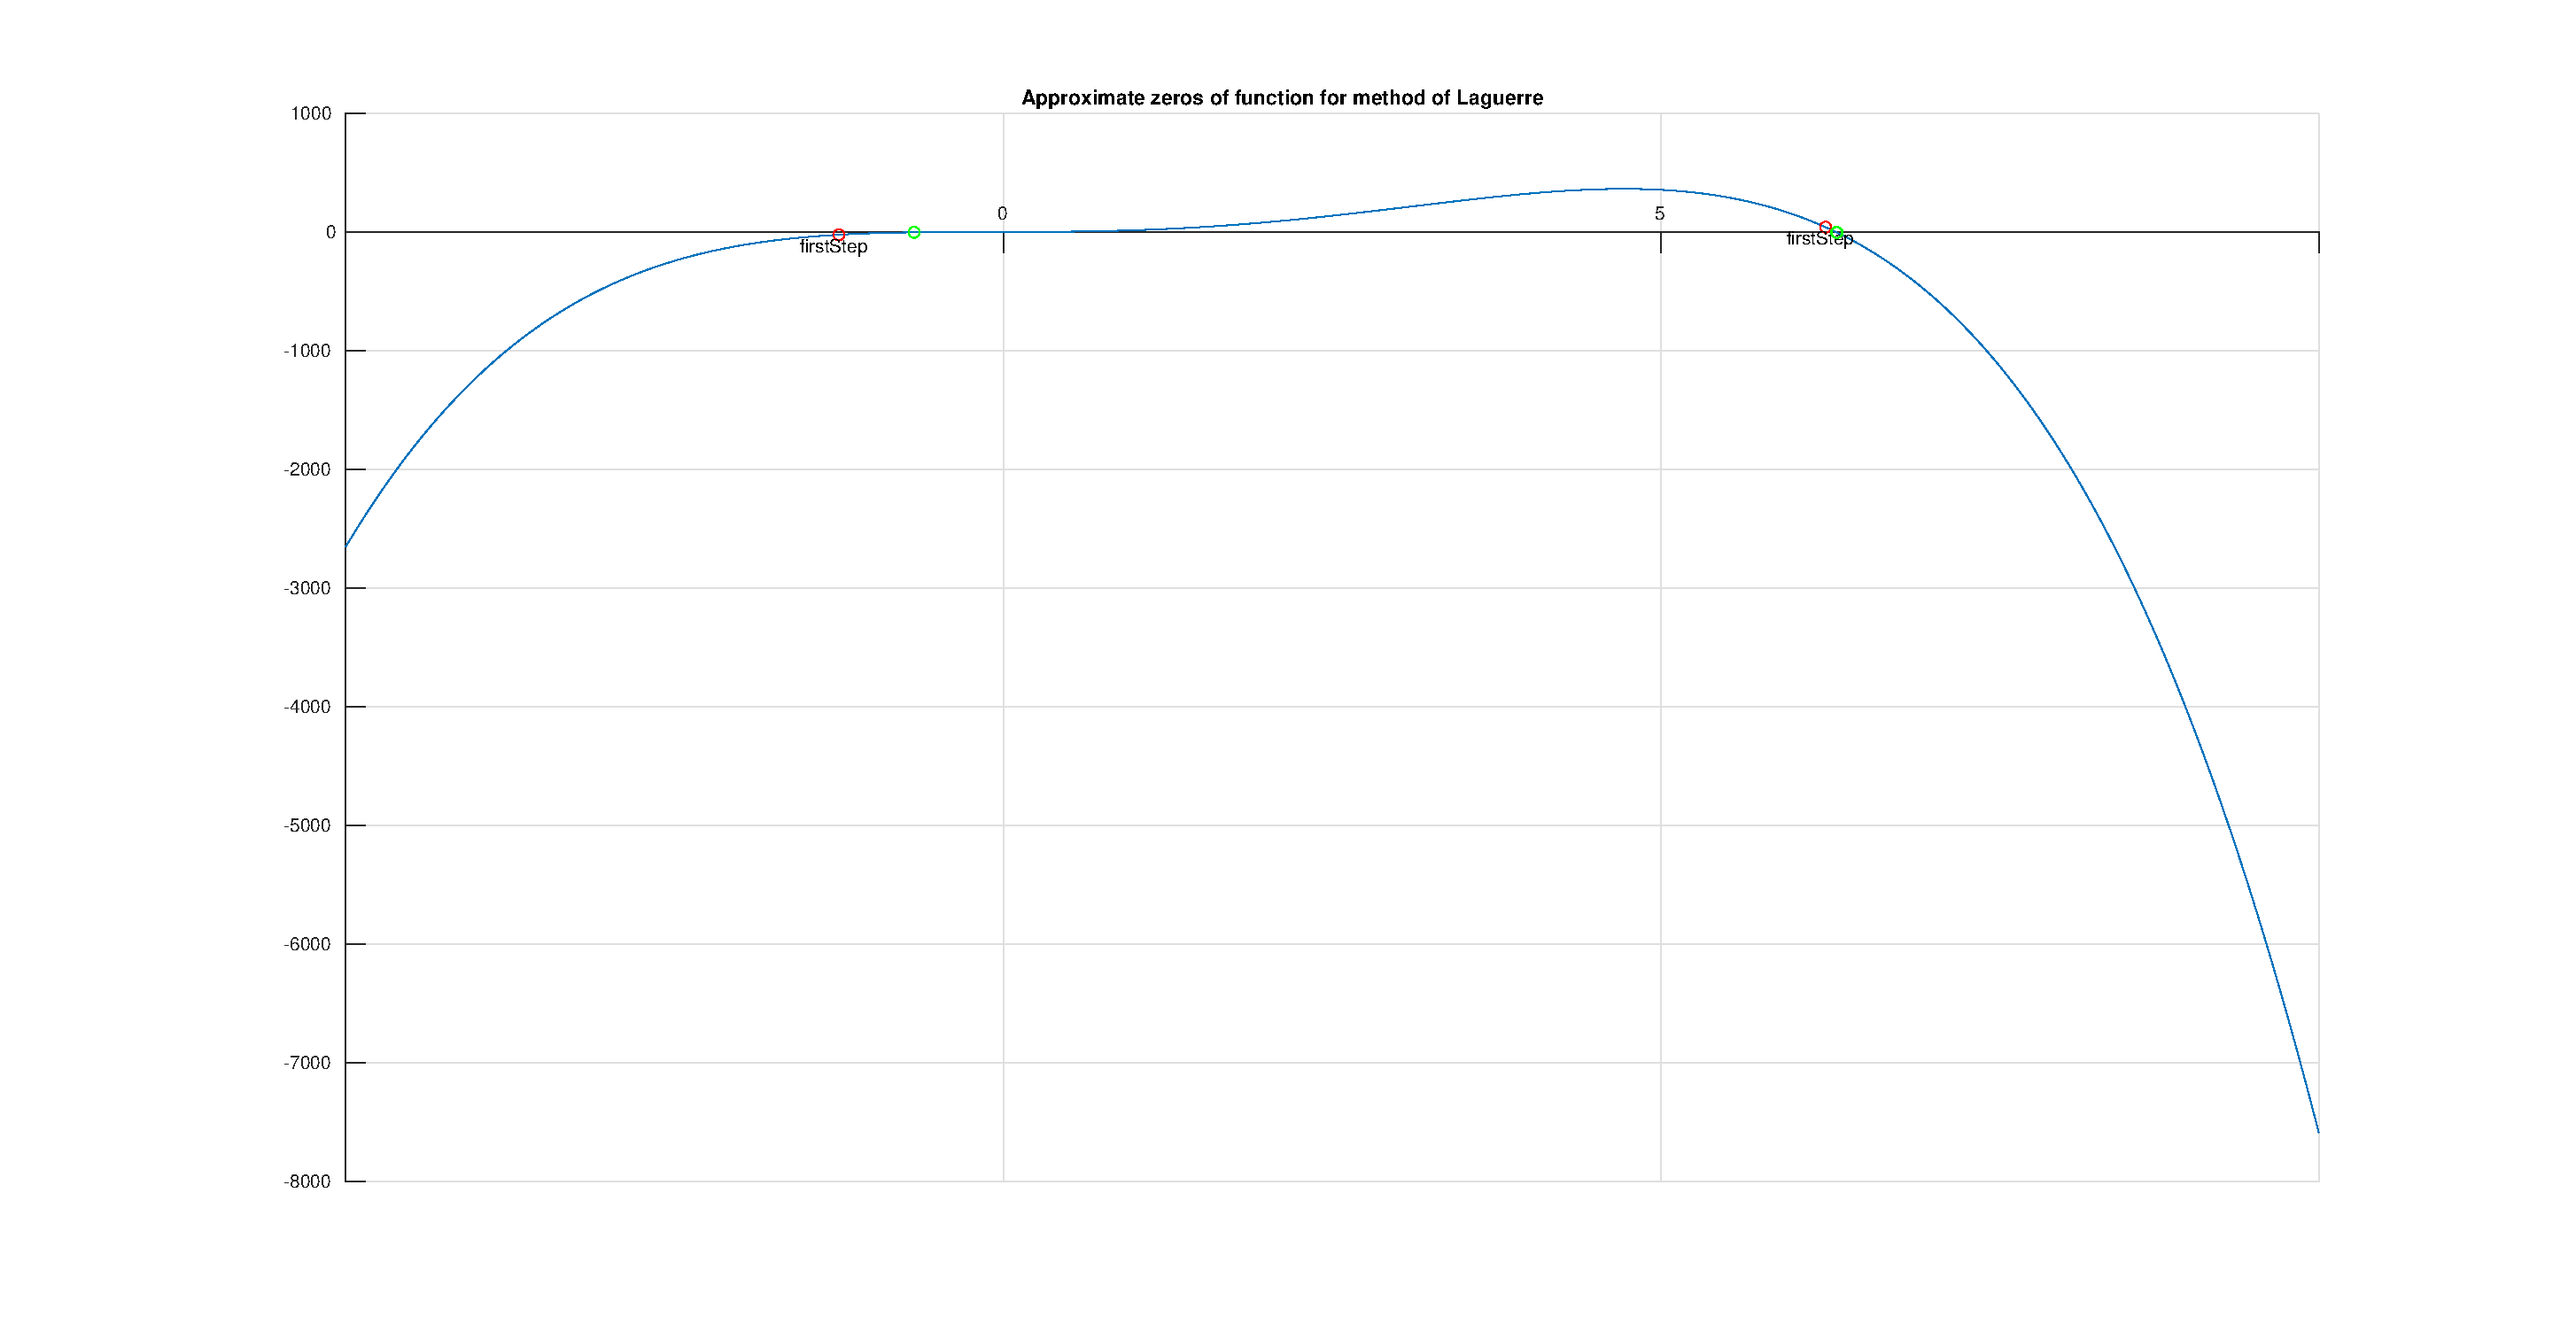
\includegraphics[scale=0.25]{task3overall.eps}
\end{center}


\begin{center}
   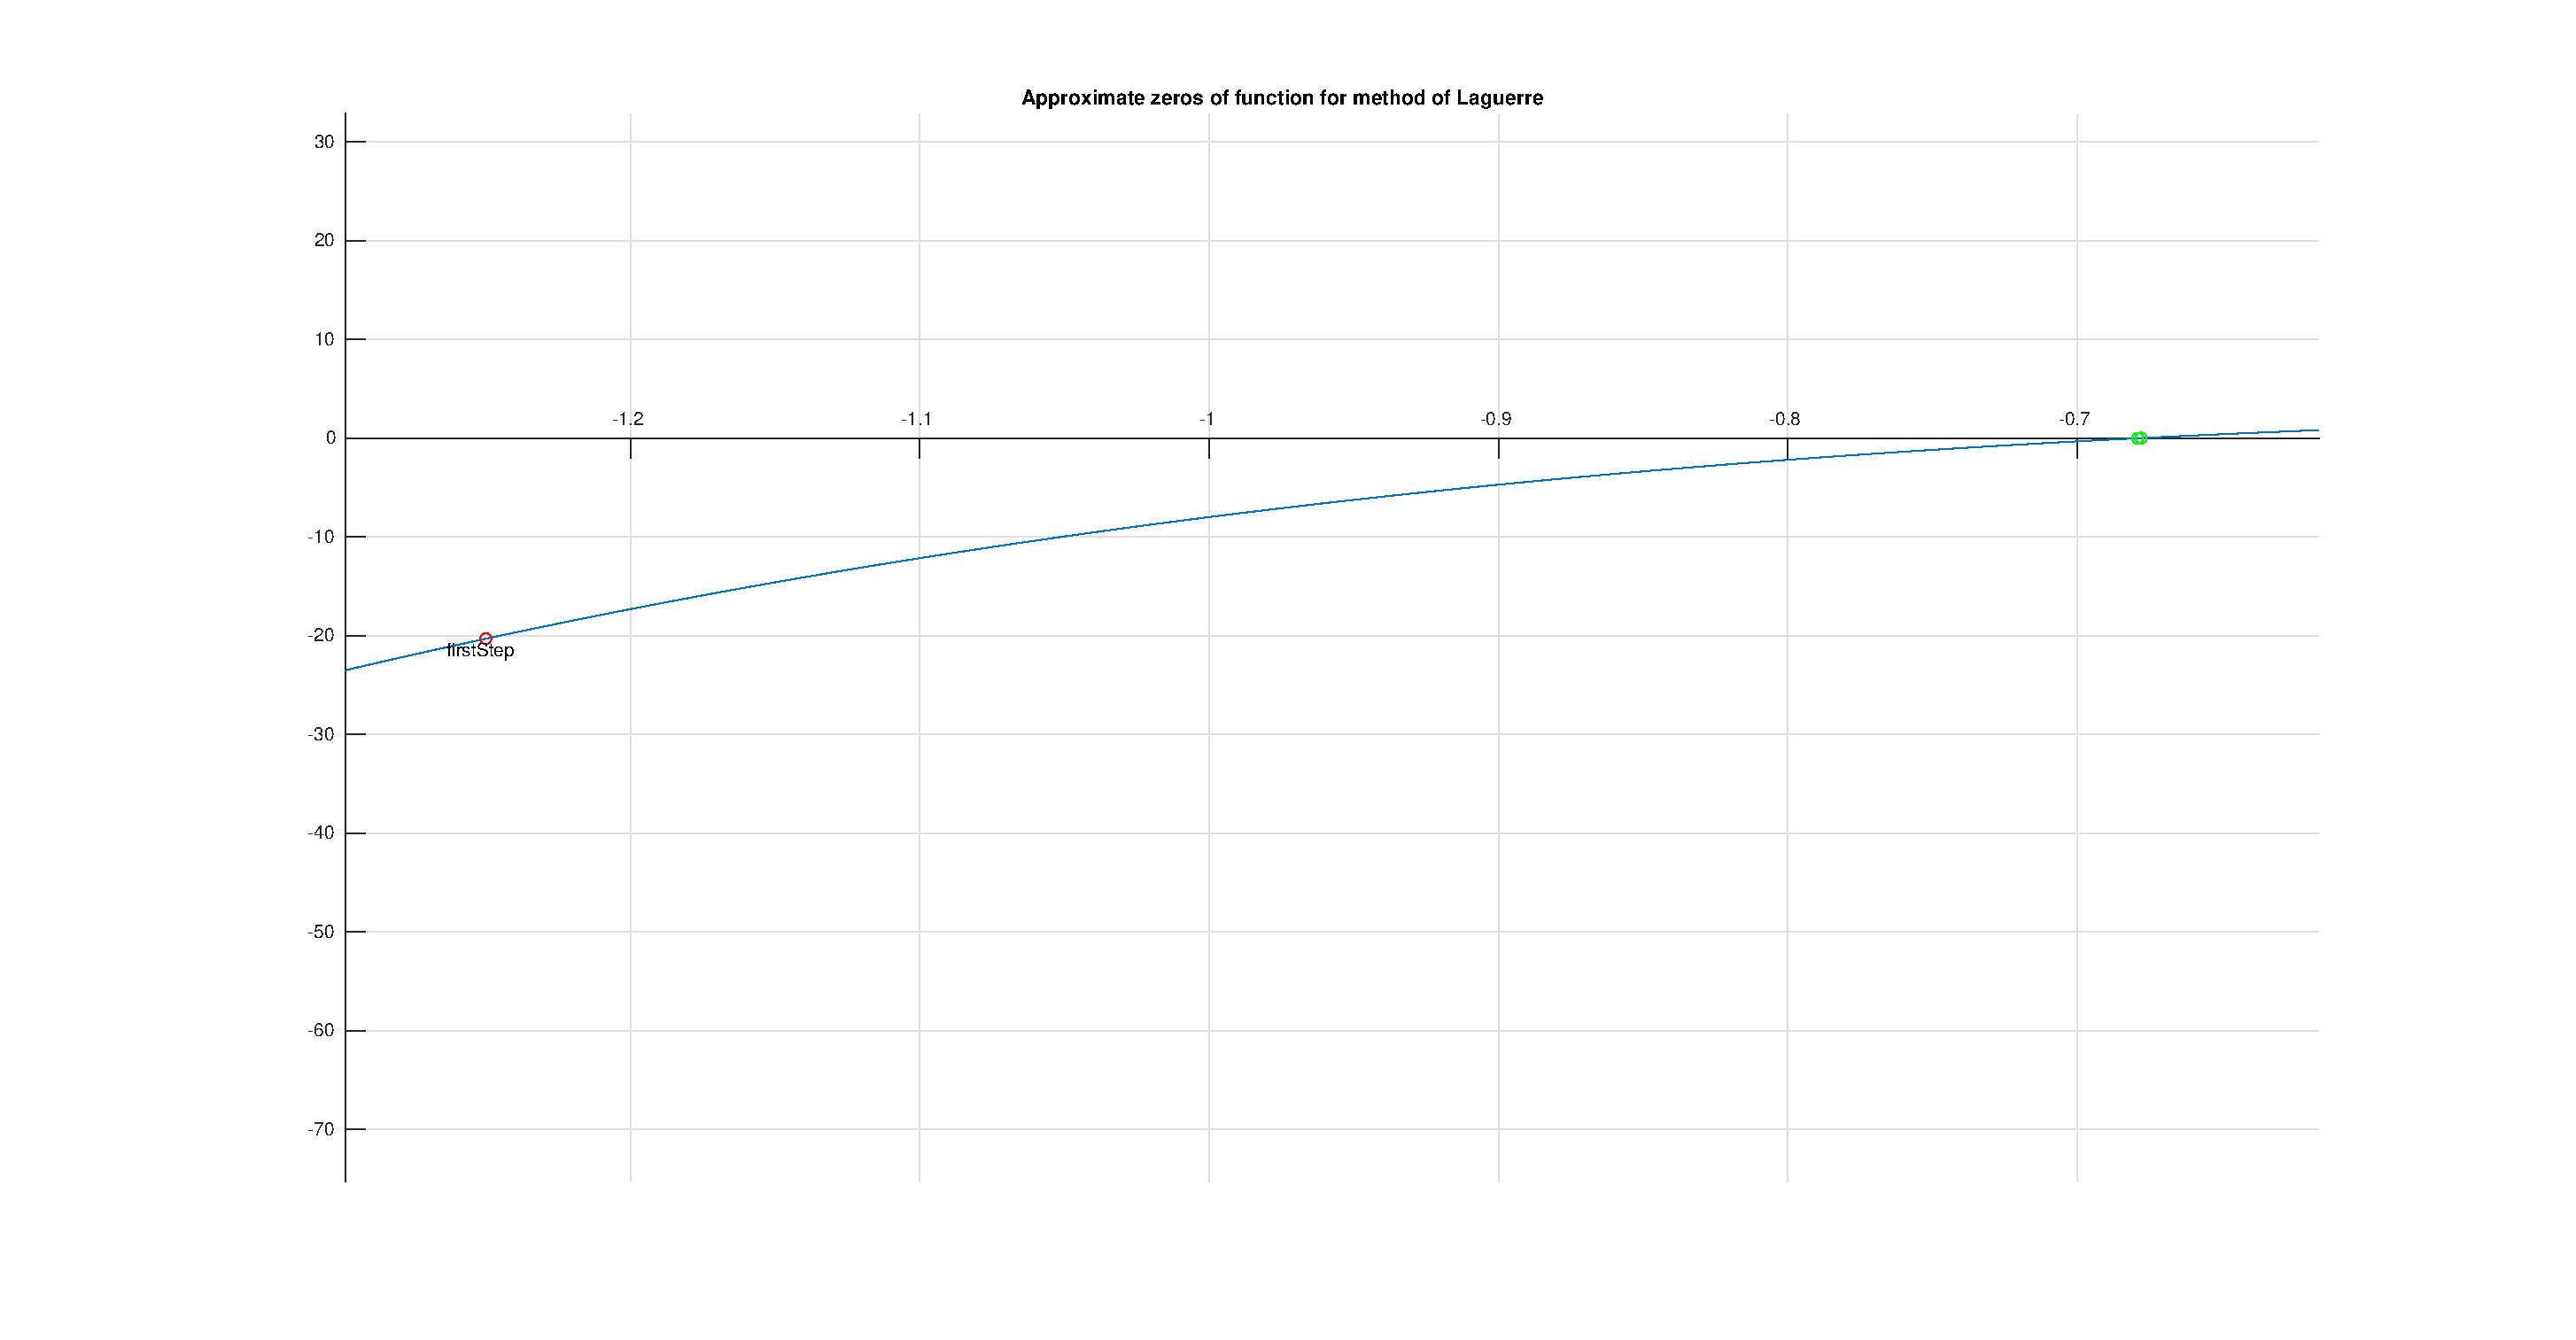
\includegraphics[scale=0.25]{task3left.eps}
\end{center}

\begin{center}
   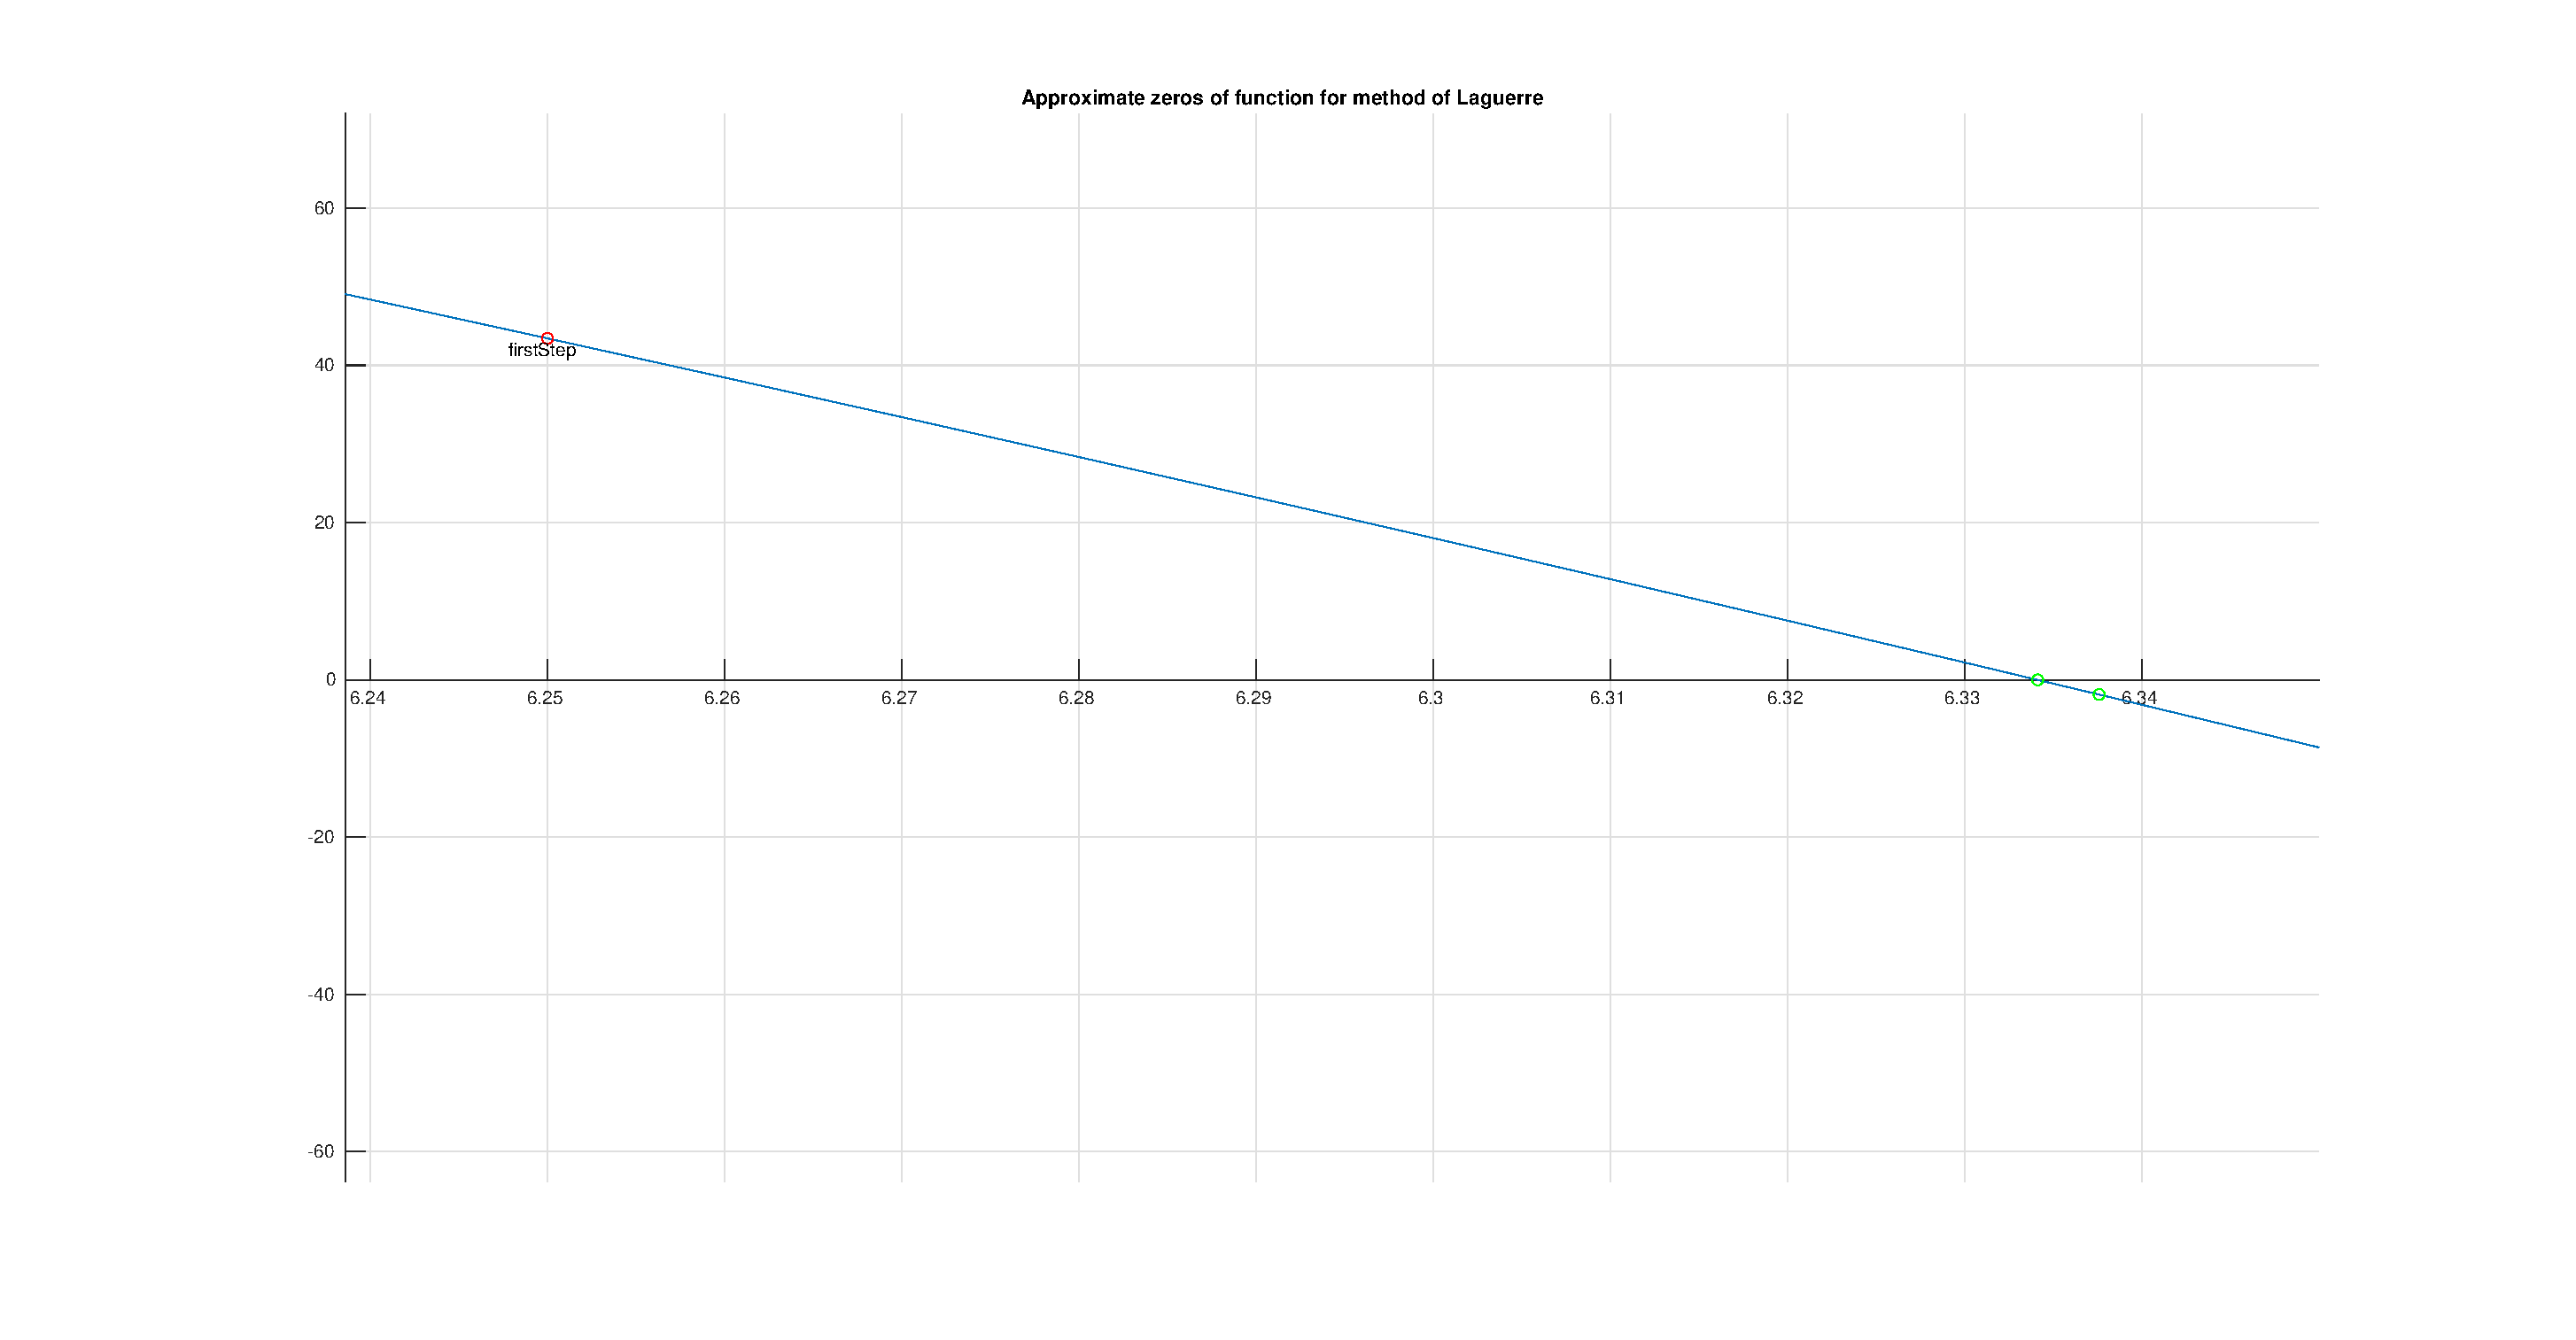
\includegraphics[scale=0.25]{task3right.eps}
\end{center}

\begin{center}
   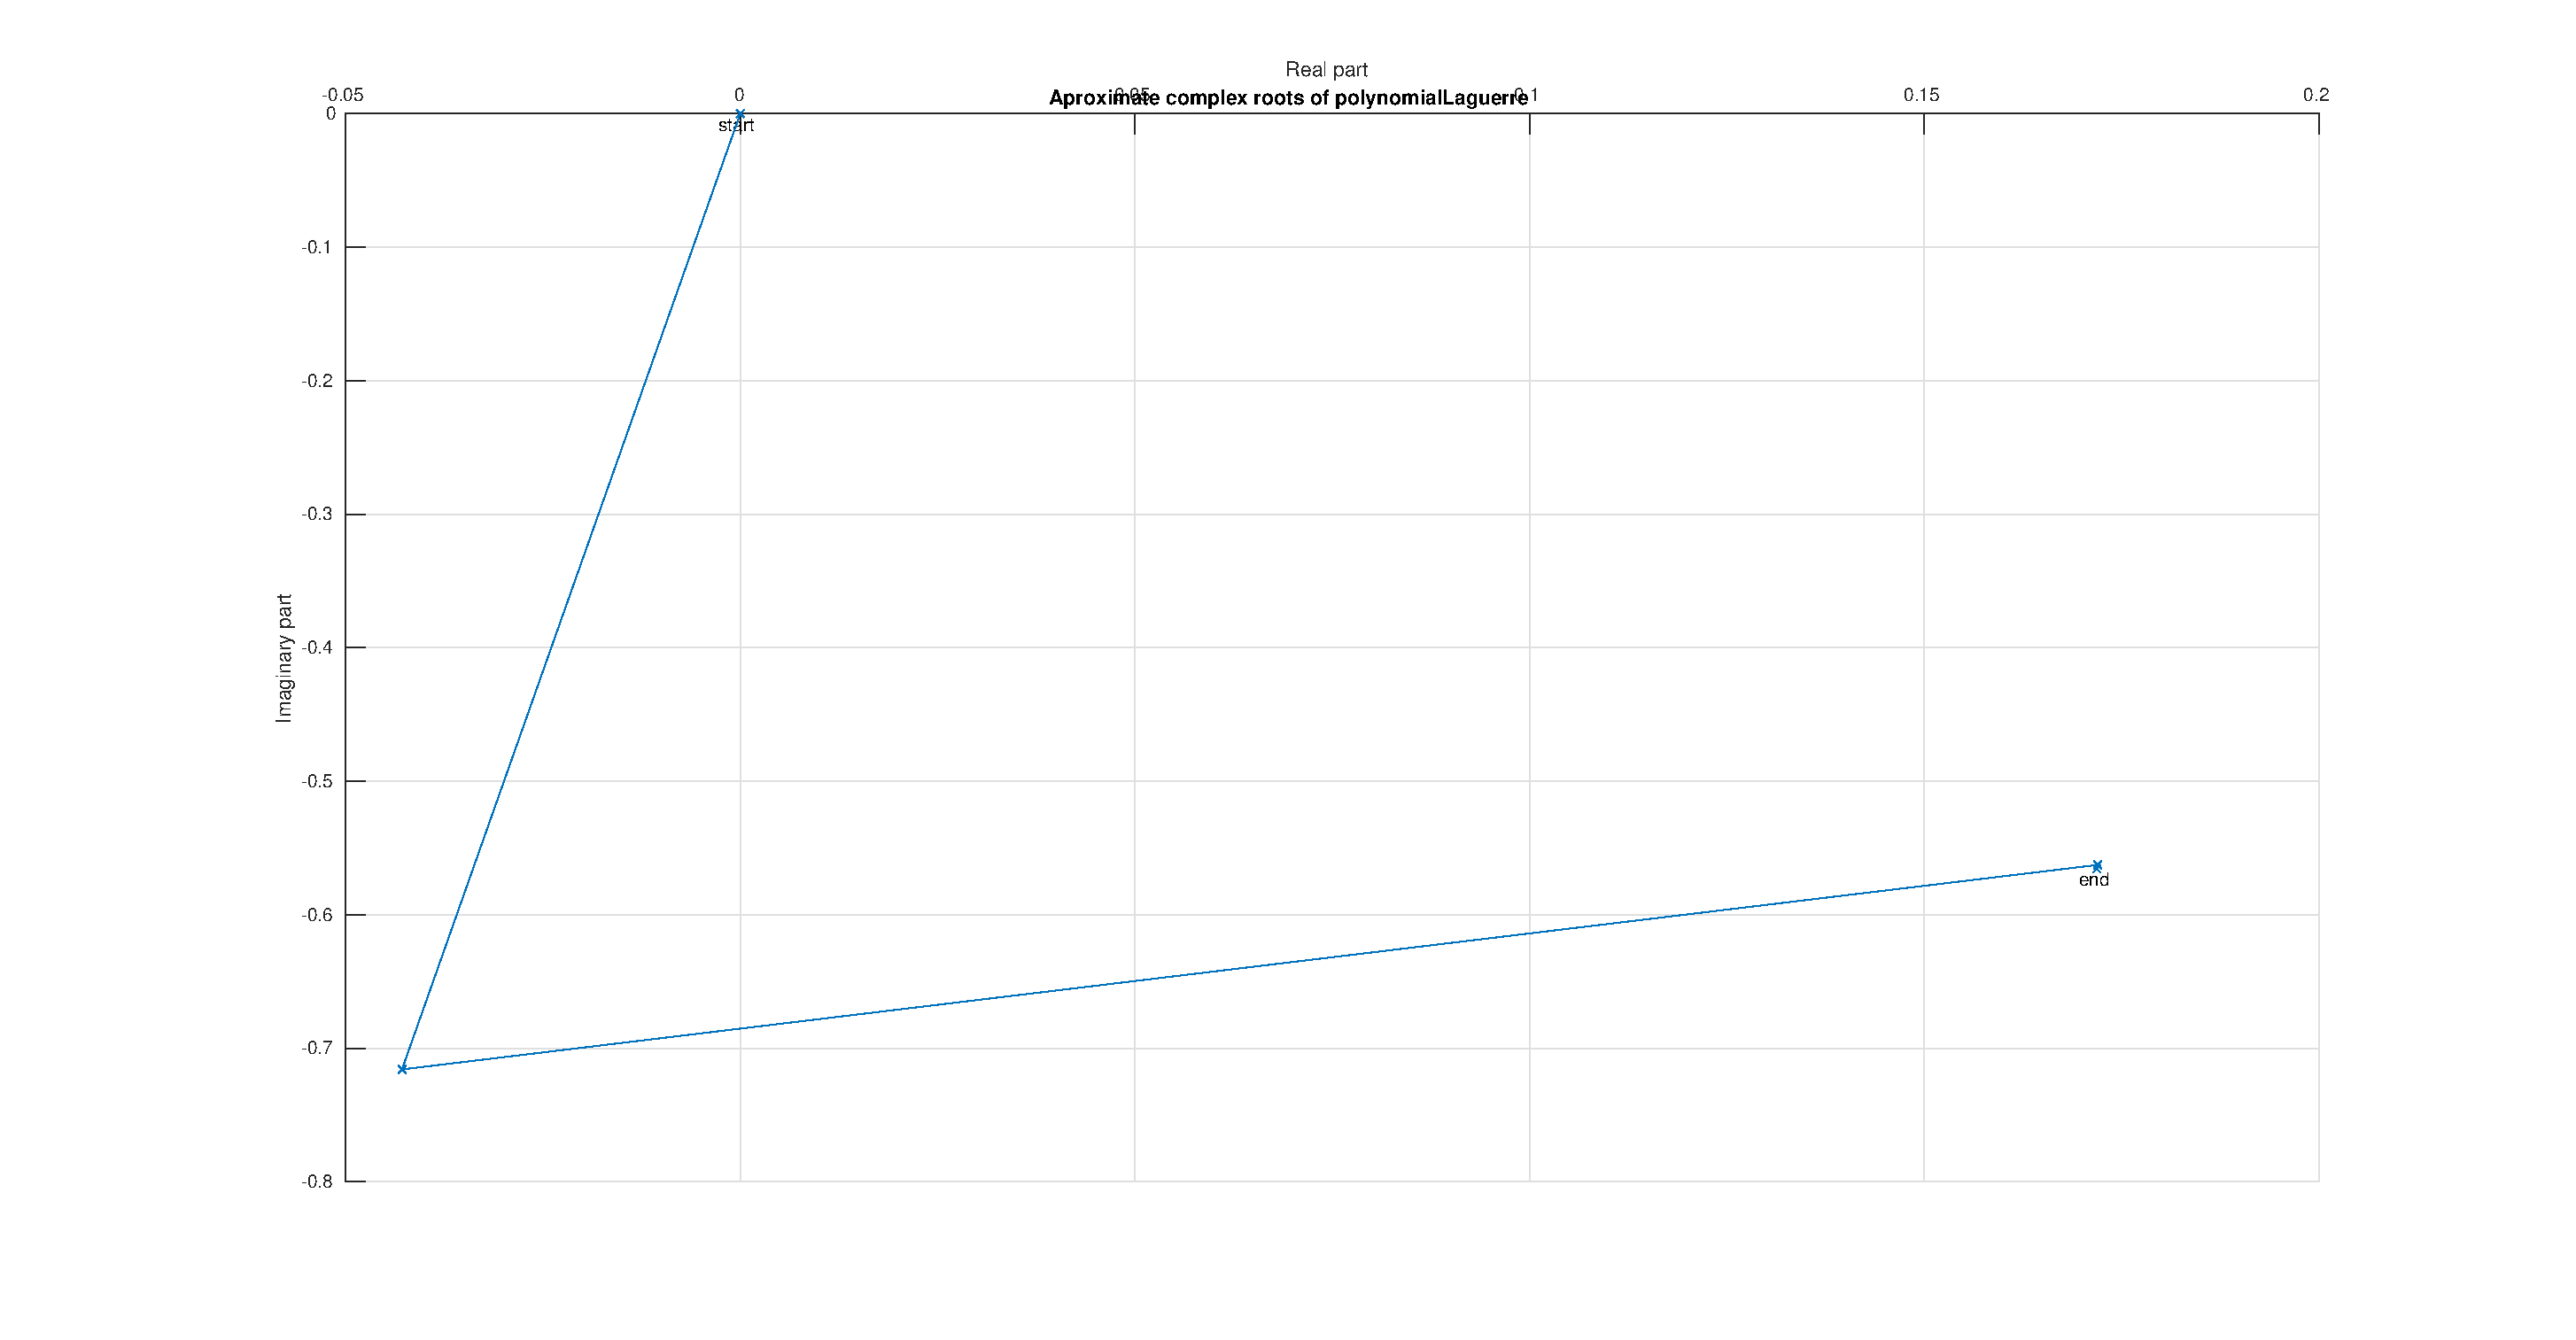
\includegraphics[scale=0.25]{task3complexoverall.eps}
\end{center}

\begin{center}
   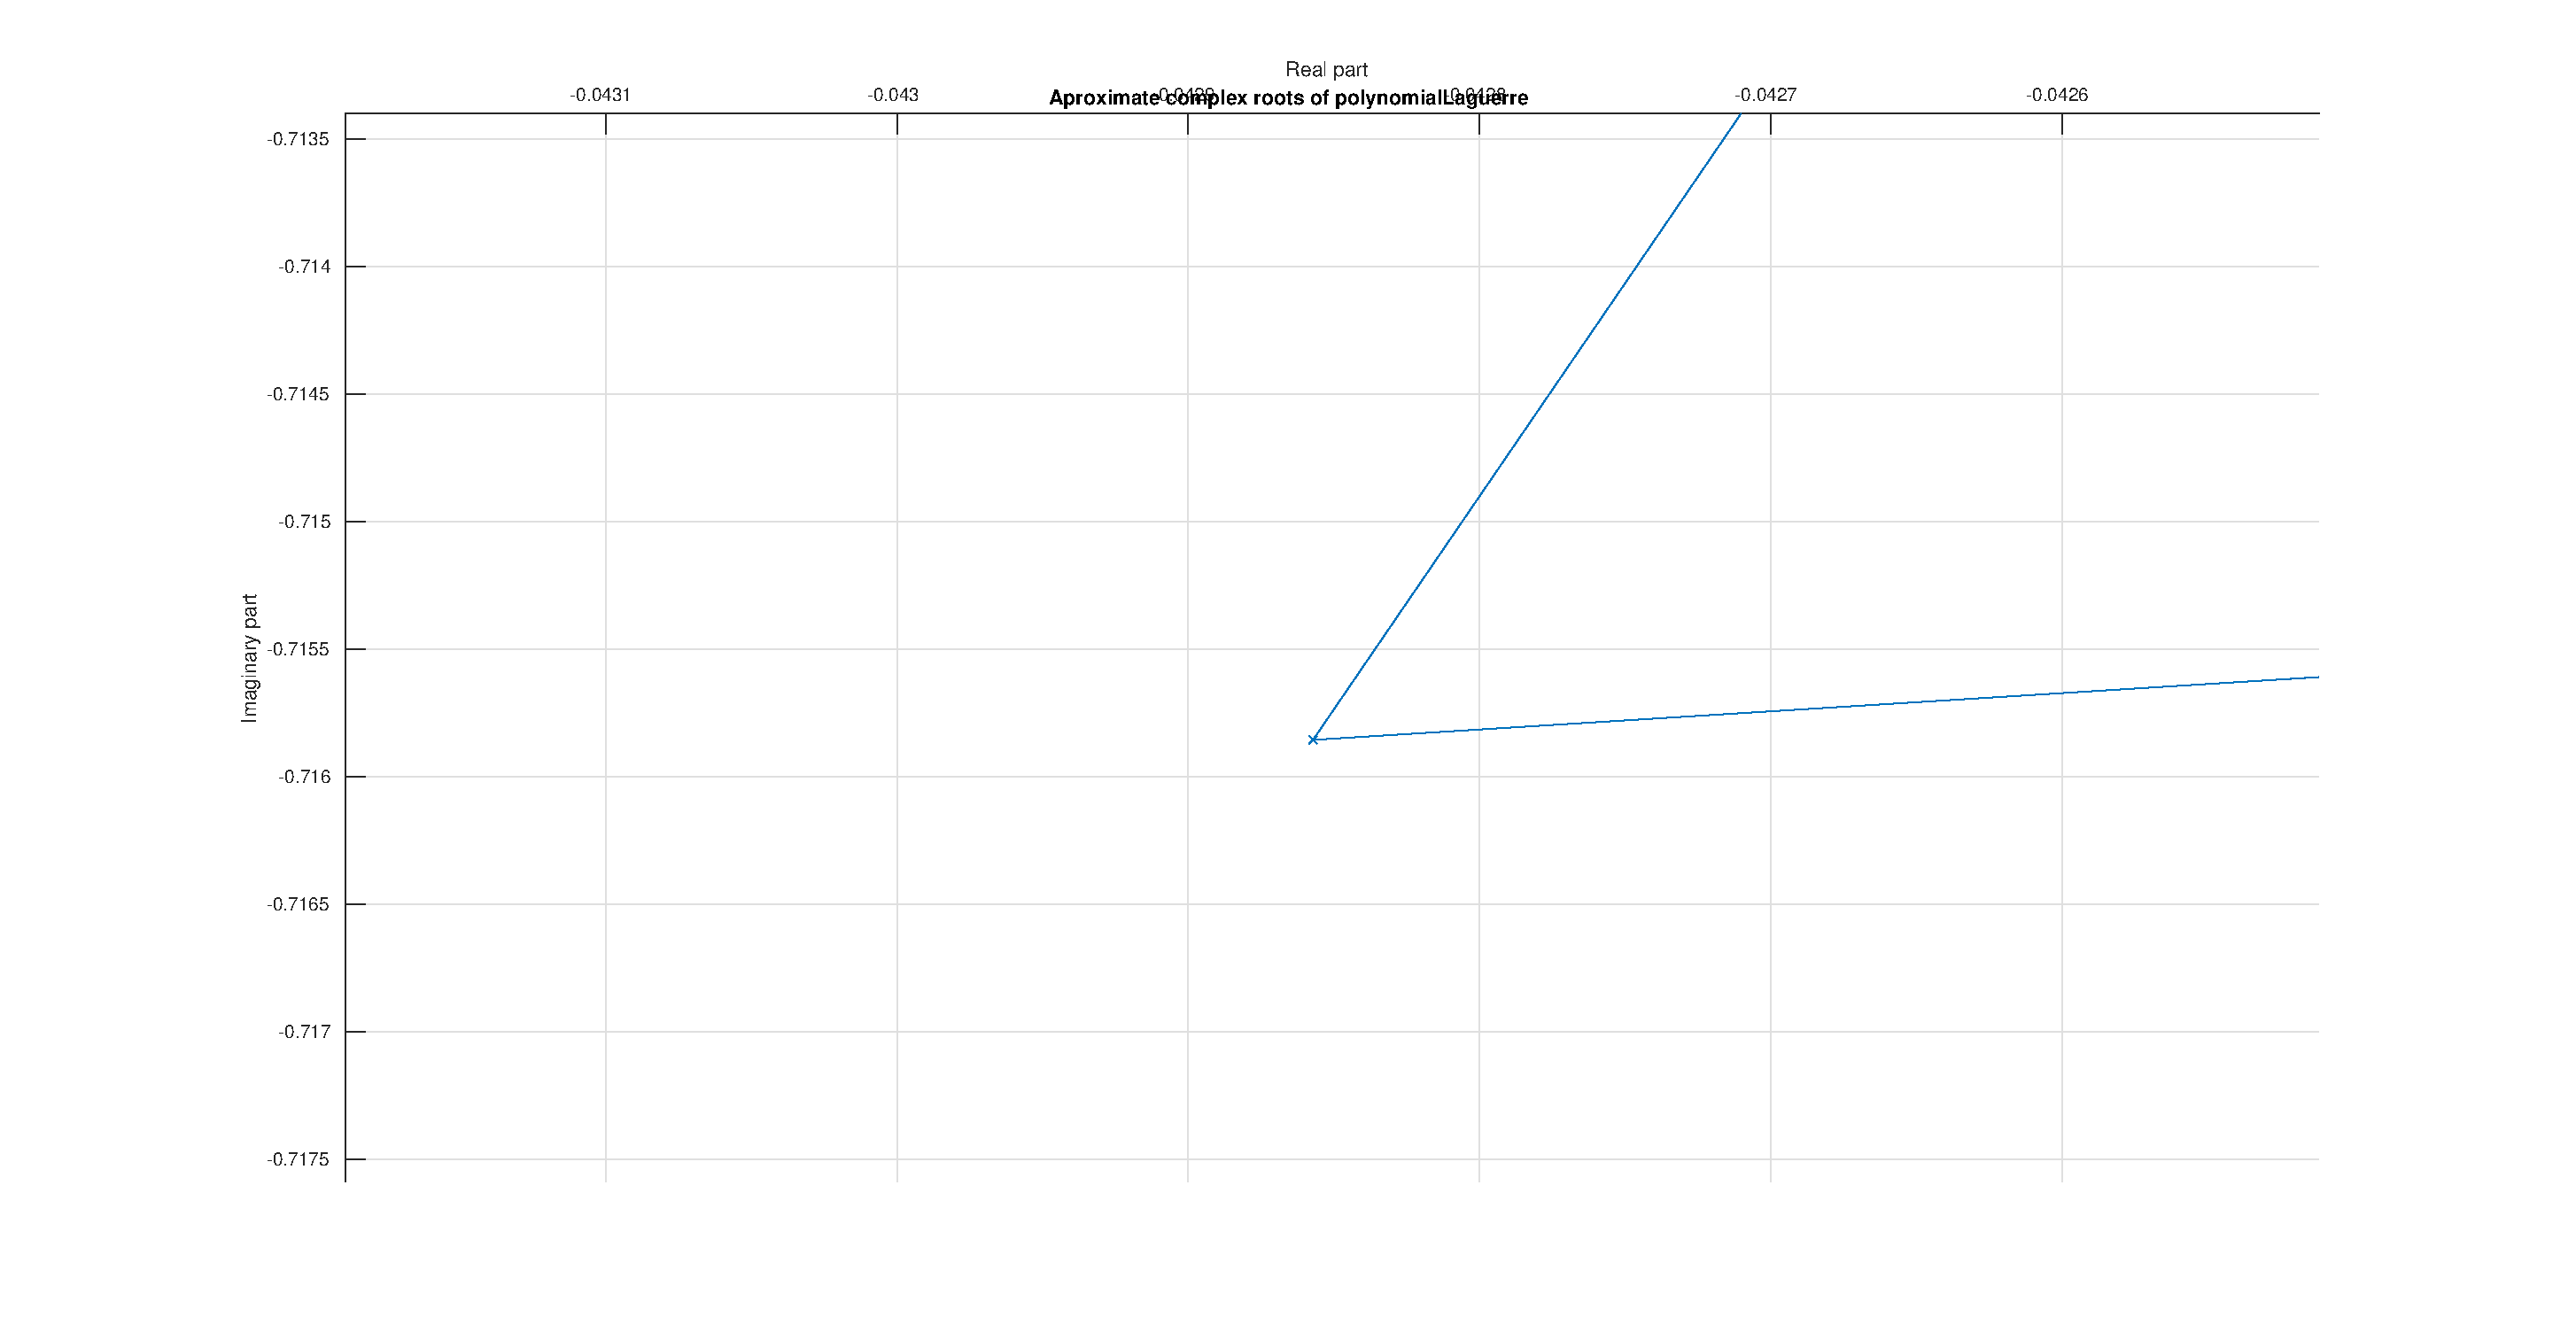
\includegraphics[scale=0.25]{task3complexleft.eps}
\end{center}

\begin{center}
   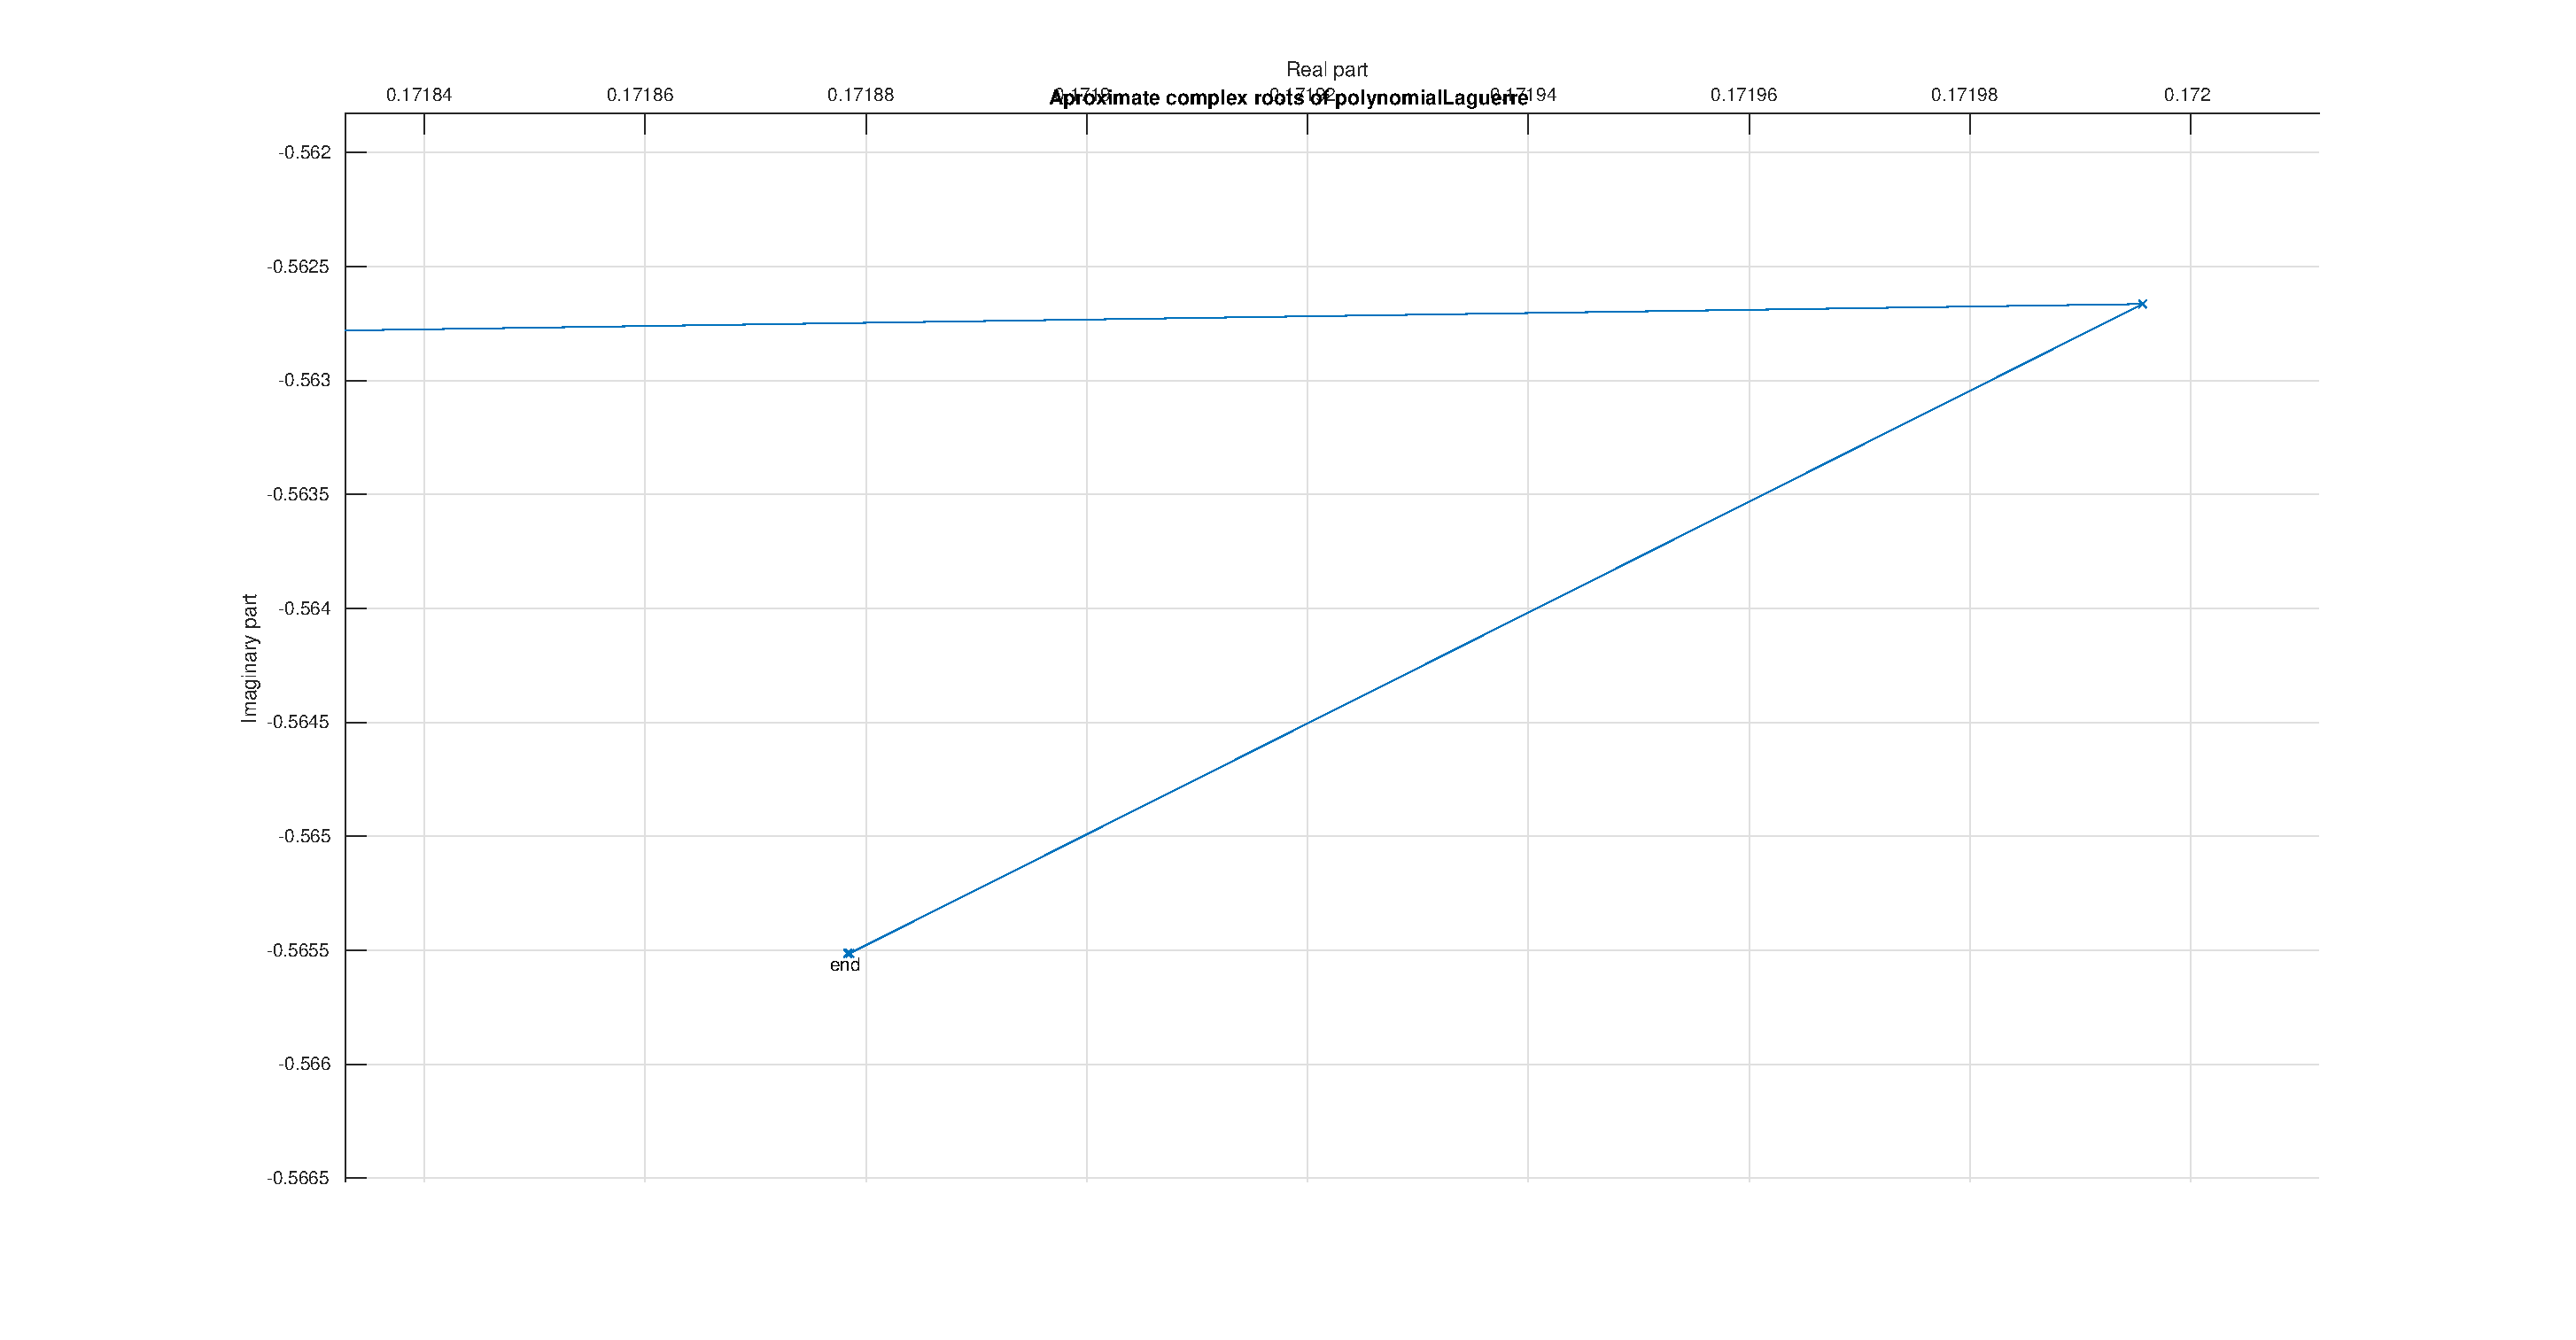
\includegraphics[scale=0.25]{task3complexright.eps}
\end{center}

\begin{center}
   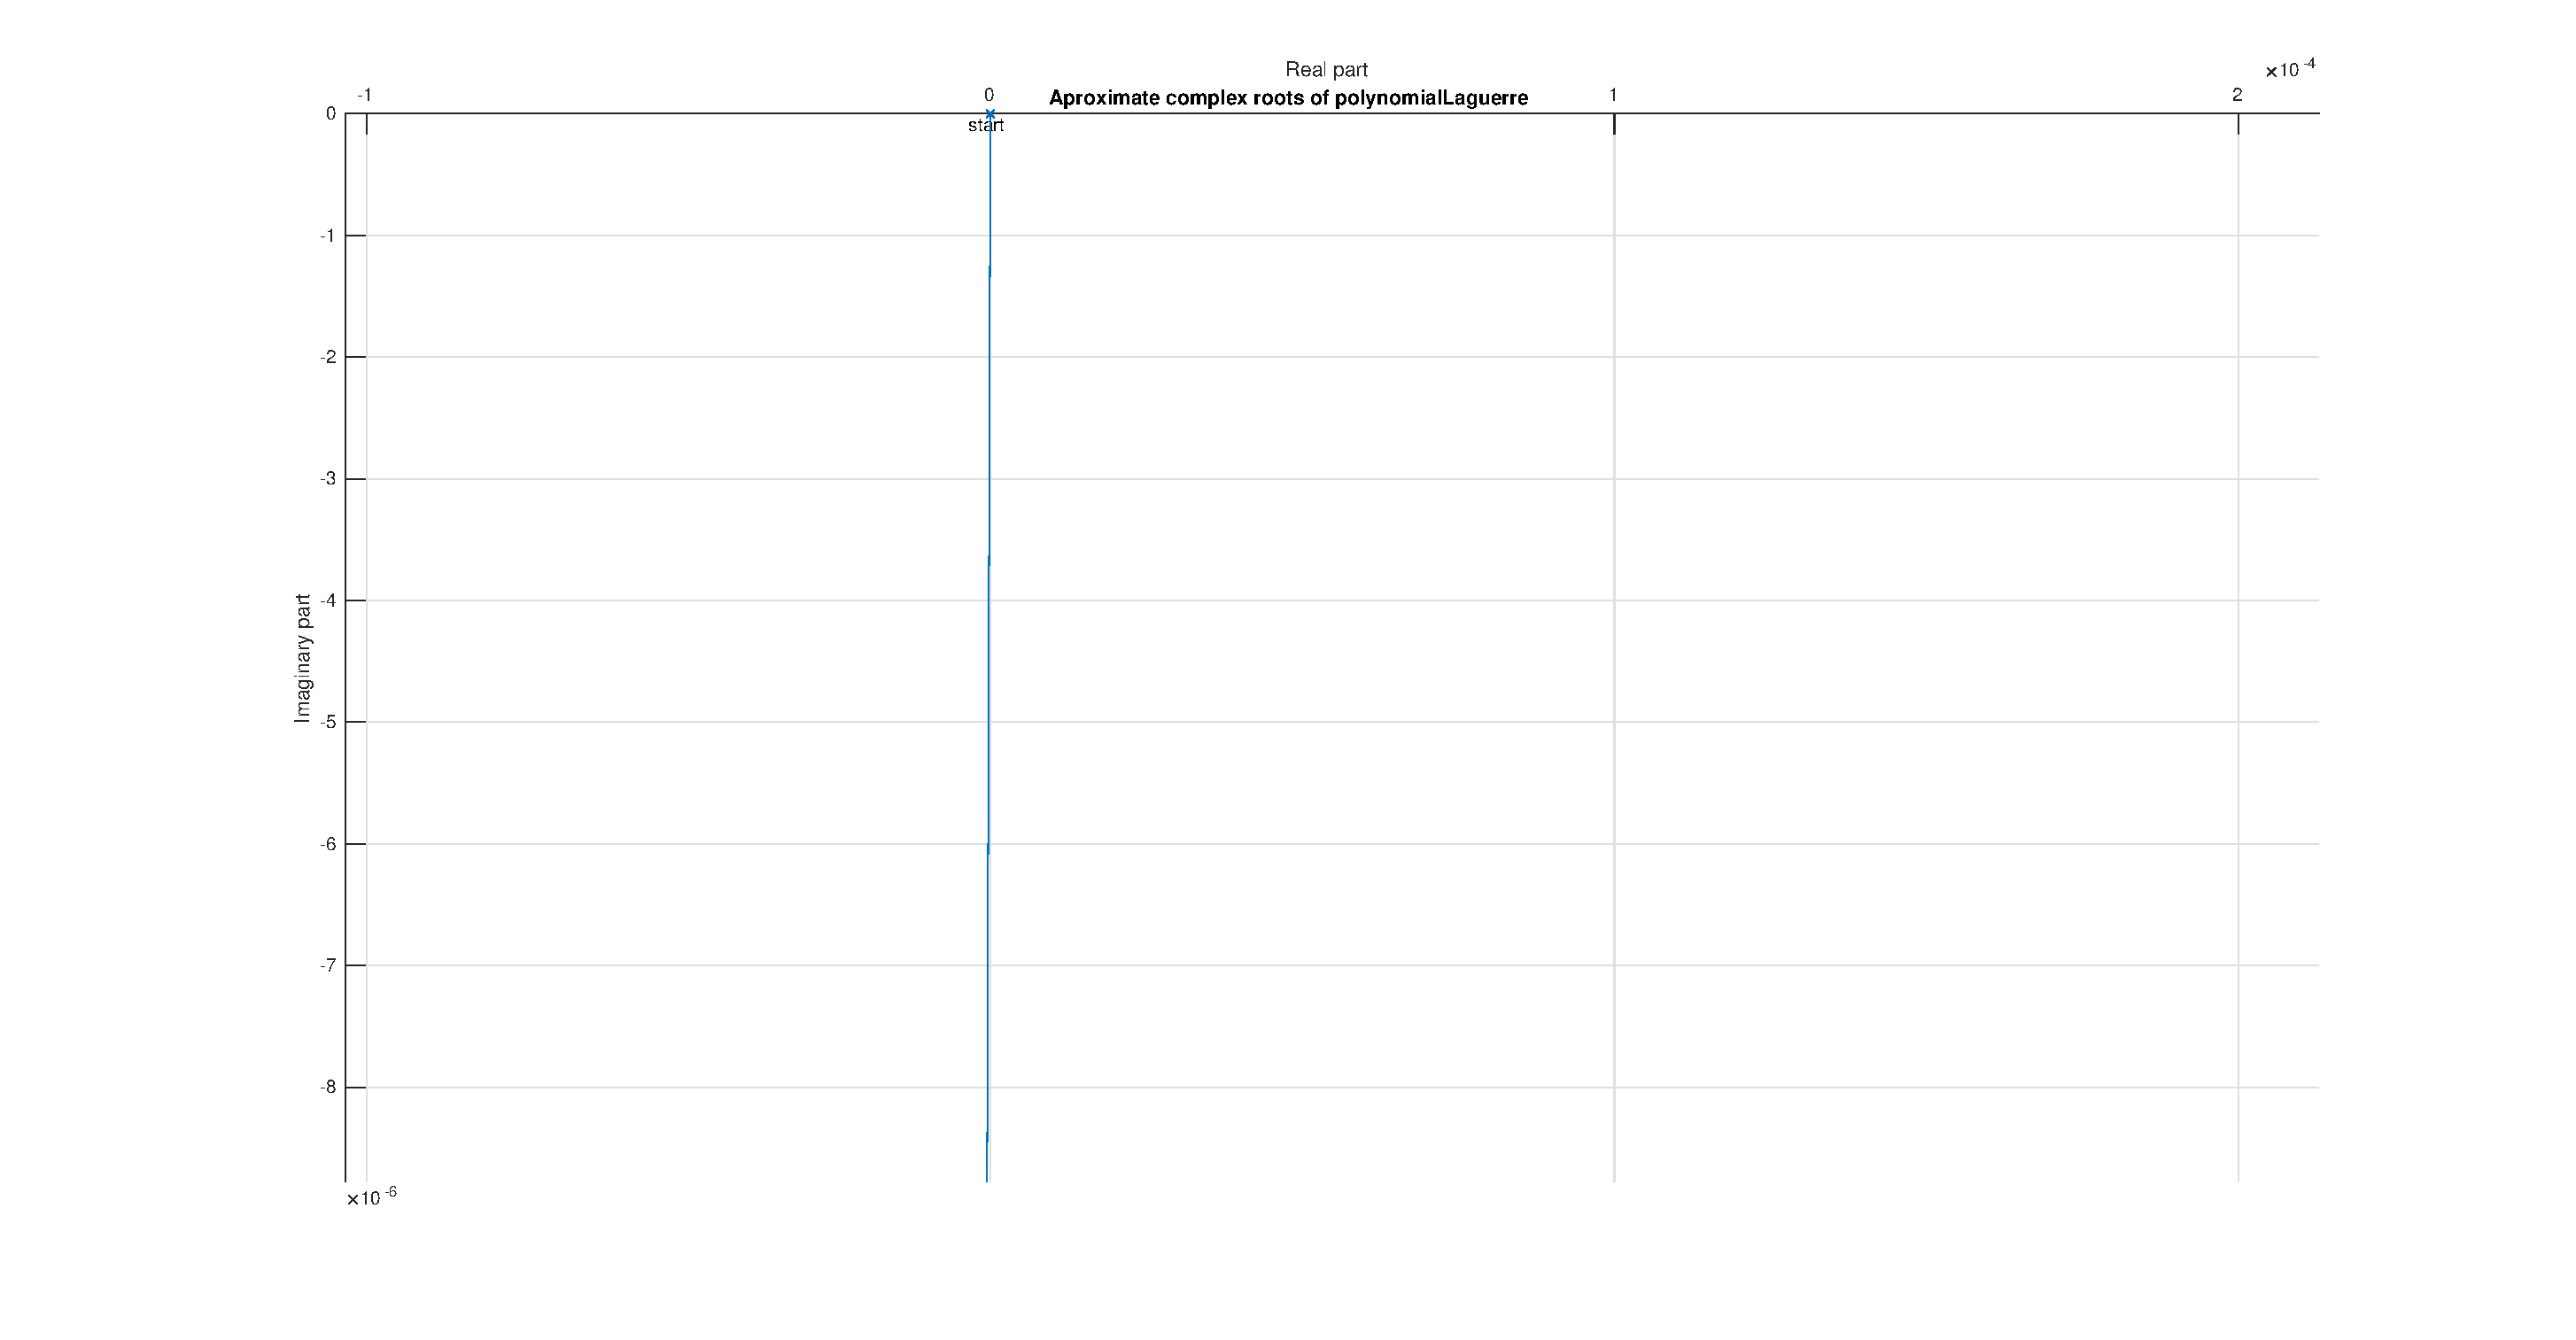
\includegraphics[scale=0.25]{task3complexup.eps}
\end{center}

\begin{center}
  \begin{tabular}{| c  c c |}
\hline
Iteration & root         & f(root) \\
\hline
1    &     -1.25   &       -20.32 \\
\hline
2    &  -0.67905   &    -0.017268 \\
\hline
3    &  -0.67787   &  -3.1489e-07 \\
\hline
4    & -0.67787    &           0 \\
\hline
\hline
\hline

\end{tabular}
\end{center}

\begin{center}
  \begin{tabular}{| c  c c |}
\hline
Iteration & root         & f(root) \\
\hline
1   &     6.25   &        43.43 \\
\hline
2   &   6.3376   &      -1.8647 \\
\hline
3   &  6.3341    &   0.0029631 \\
\hline
4   &   6.3341   &  7.9942e-09\\
\hline
5   &  6.3341    & -7.1942e-14\\
\hline


\end{tabular}
\end{center}


\begin{center}
  \begin{tabular}{| c  c c |}
\hline
Iteration & root         & f(root) \\
\hline
1   &           0+0i           &           3 \\
\hline
2   &   -0.042857+0.71586i     &      4.1826 \\
\hline
3   &       0.172+0.56266i     &    0.040584 \\
\hline
4   &    0.17188+0.56551i     &  2.8484e-06 \\
\hline
5   &     0.17188+0.56551i    &   2.2952e-14 \\
\hline
6   &     0.17188+0.56551i    &            0 \\
\hline


\end{tabular}
\end{center}


\subsection{Comparison of results between Laguerre's method and MM2 method}

\subsubsection{Tables for MM2}

\begin{center}
  \begin{tabular}{| c  c c |}
\hline
Iteration & root         & f(root) \\
\hline
1  &       -1.25+0i         &         -20.32+0i    \\
\hline
2  &    -0.72604-0.25326i   &         1.0515-4.0744i  \\
\hline
3  &   -0.68613-0.01483i    &      -0.11667-0.22303i   \\
\hline
4  &   -0.67788+2.5407e-06i &   -0.00010163+3.7123e-05i \\
\hline
5  &    -0.67787-8.0819e-13i &    1.4105e-11-1.1809e-11i \\
\hline
 \hline

\end{tabular}
\end{center}

\begin{center}
  \begin{tabular}{| c  c c |}
\hline
Iteration & root         & f(root) \\
\hline
1   &     6.25    &       43.43 \\
\hline
2   &   6.3376    &     -1.8647 \\
\hline
3   &  6.3341     &  0.0029695 \\
\hline
4   &   6.3341    &  1.6294e-08 \\
\hline
5   &   6.3341    & -4.6896e-13 \\
\hline
\hline

\end{tabular}
\end{center}

\begin{center}
  \begin{tabular}{| c  c c |}
\hline
Iteration & root         & f(root) \\
\hline
1   &         0+0i          &            3 \\
\hline
2   &    -0.125+0.85696i    &       8.0341 \\
\hline
3   &   0.16892+0.62593i    &      0.94053 \\
\hline
4   &   0.17203+0.56536i    &    0.0031354  \\
\hline
5   &   0.17188+0.56551i    &   3.8615e-09  \\
\hline
6   &   0.17188+0.56551i    &            0  \\
\hline
\hline

\end{tabular}
\end{center}

As expected Laguerre's method reigns supreme, it is:
\begin{enumerate}
\item Faster
With 5 iterations on average compared to around 5.3 for MM2
\item More accurate
For real root -0.67787 matlab calculated the value of this function for Laguerre's method as equal to exactly 0 as opposed to around $10^{-11}$ error for MM2.
\item With no errors
Laguerre's method did not mistakenly added imaginary part to real root -0.67787 as MM2 did. 
\end{enumerate}

Laguerre's method is faster and more accurate than MM2 which means that we can compare it to faster version of MM1, this means that it is the best method we tested in this exercise.

\chapter{Code appendix}

